\documentclass[a4paper, 11pt]{article}

\usepackage{floatrow}
\usepackage{physics}
\usepackage{xcolor}
\usepackage{amsfonts}
\usepackage{graphicx}
\usepackage{multirow}
\usepackage{amsmath}
\usepackage{mathtools}
\usepackage{ragged2e}
\usepackage{esint}
\usepackage{wrapfig}
\usepackage{mdframed}
\usepackage{filecontents}
\usepackage{lipsum} 
\usepackage{pdflscape}
\usepackage{lscape}
\usepackage{caption}
\usepackage{subcaption}
\usepackage{hyperref}
\usepackage{bm}
\usepackage{booktabs}
\usepackage{dcolumn}% Align table columns on decimal point
\usepackage{minted}
\definecolor{codegreen}{rgb}{0,0.6,0}
\definecolor{codegray}{rgb}{0.5,0.5,0.5}
\definecolor{codepurple}{rgb}{0.58,0,0.82}
\definecolor{backcolour}{rgb}{0.95,0.95,0.92}
\definecolor{bg}{HTML}{282828}
\usemintedstyle{monokai}
\newfloatcommand{capbtabbox}{table}[][\FBwidth]

%\addbibresource{reference.bib}

\begin{document}
\title{SKKU 2024 Challenge: Heisenberg Spin Glass}
\author{Donghun Jung}
\maketitle

\section*{Part I : A first look at the Heisenberg spin glass}

\subsection*{How many symmetry classes are there?}
There are 11 distinct symmetry classes, each characterized by unique eigenspectra. 
I conducted eigen-decomposition for all 64 possible combinations of the coefficients $J_{ij}$. 

The following code generates the Heisenberg Hamiltonian $H_{heisenberg}$:
\begin{minted}[bgcolor=bg,
  frame=lines,
  framesep=2mm]{python}
def __reset__(self):
    qubit_idx = [idx for idx in range(self.num_qubits)]
    combinations = itertools.combinations(qubit_idx, 2)
    
    H_z = np.zeros([2**self.num_qubits, 2**self.num_qubits]
                    , dtype=np.complex128)
    if self.coefficients2 is not None:
        for i in range(self.num_qubits):
            temp = [self.I for _ in range(self.num_qubits)]
            temp[i] = self.Pauli_Z
            H_z += self.coefficients2[i]*self._Kron(temp)
    
    H_heisenberg = np.zeros([2**self.num_qubits, 
                            2**self.num_qubits]
                            , dtype=np.complex128)
    for coefficient, pair_idx 
      in zip(self.coefficients1, combinations):
        H_heisenberg += coefficient * self._H_ij(pair_idx)
    self.H_sg = H_heisenberg + H_z
\end{minted}

In this example, \texttt{self.coefficients2} is set to \texttt{None}. 
Within the \texttt{for} loop, each pair of qubit indices $(i,j)$ runs through unique combinations in the following sequence: 
$(0,0)$, $(0,1)$, $(0,2)$, $(1,2)$, $(1,3)$, $(2,3)$.
This setup ensures that each distinct interaction between qubits is included without repetition, 
covering all possible unique two-qubit interactions in the Heisenberg Hamiltonian $H_{heisenberg}$.
Additionally, the \texttt{\_Kron} method is implemented to maintain the Qiskit bit-ordering convention.
\begin{minted}[bgcolor=bg,
  frame=lines,
  framesep=2mm]{python}
def _Kron(self, array):
    prod = np.array(1)
    if len(array) == 0:
        return prod
    else:
        for element in array:
            prod = np.kron(element, prod) 
        return prod
\end{minted}

Two models are classified within the same symmetry class if their eigenspectra are identical. 
Here, the eigenspectrum of a Hamiltonian represents the set of its eigenvalues. To numerically determine whether two eigenspectra are equivalent, I used the \texttt{np.allclose} function.
\begin{minted}[bgcolor=bg,
  frame=lines,
  framesep=2mm]{python}
symmetry_classes = {}
for coefficient_combination 
  in itertools.product([1, -1], repeat=6):

    eigenspectrum = H_sg(coefficient_combination, [0, 0, 0, 0])
    symmetry_classes[coefficient_combination] = eigenspectrum

classified_groups = {}
unique_eigenspectra = {}
class_count = 0

for combination, spectrum in symmetry_classes.items():
  is_duplicate = False
  for class_id, class_spectrum in unique_eigenspectra.items():
    if np.allclose(class_spectrum, spectrum._eigenSpectrum()):
      is_duplicate = True
      classified_groups[class_id].append(combination)
      break

  if is_duplicate:
    continue
  else:
    class_count += 1
    classified_groups[class_count] =[combination]
    unique_eigenspectra[class_count]=spectrum._eigenSpectrum()
\end{minted}

Detailed information on eigenspectra and coefficient values can be found in the next questions.

\subsection*{For each symmetry class, provide one set of $J_{ij}$ coefficients for a model in that symmetry class.}

The Heisenberg Hamiltonian $\mathcal{H}_{\text{heisenberg}}$ is defined as:
\begin{equation}
  \mathcal{H}_{\text{heisenberg}} = \sum_{(i,j)} J_{i,j} H_{i,j}
\end{equation}
where
\begin{equation}
  H_{i,j} = \sigma_x^i \sigma_x^j + \sigma_y^i \sigma_y^j + \sigma_z^i \sigma_z^j 
\end{equation}
The interaction is ferromagnetic when $J_{ij} = 1$ and anti-ferromagnetic when $J_{ij} = -1$. 
This Hamiltonian pocesses intrinsic symmetry: Interchange symmetry. 
Under the interchange interaction on qubit $i$ and $j$, both of Hamiltonian eigenvalues and eigenstates remain unchanged. 
Therefore, the elements in the same symmetry class can be generated via interchange operation. 

The blue edge denotes ferromagnetic interaction and red edge denotes anti-ferromagnetic interaction.

\begin{figure}[h]
  \centering
  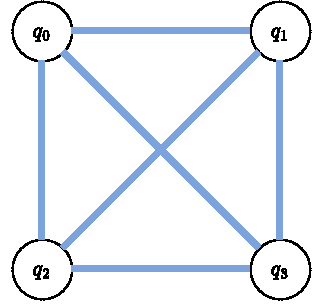
\includegraphics[width=0.5\textwidth]{./figure/class1.pdf}
  \caption{caption}
\end{figure}

\begin{table}[!h]
  \begin{tabular}{cccccc}
    \toprule\toprule
    $J_{01}$ & $J_{02}$ & $J_{03}$ & $J_{12}$ & $J_{13}$ & $J_{23}$ \\ 
    \midrule
    $1$ & $1$ & $1$ & $1$ & $1$ & $1$  \\
    \bottomrule
    \caption{Example LaTeX Table} 
    \label{tab:example1}
  \end{tabular}
\end{table}
\paragraph{Class 1. } The whole interactions are ferromagnetic. There is no other possible element even by using interchange interaction. 

Class 2


\begin{table}[!h]
  \begin{tabular}{cccccc}
    \toprule\toprule
    $J_{01}$ & $J_{02}$ & $J_{03}$ & $J_{12}$ & $J_{13}$ & $J_{23}$ \\ 
    \midrule
    $1$ &$1$ &$1$ &$1$ &$1$ &$-1$   \\
    $1$ &$1$ &$1$ &$1$ &$-1$ &$1$   \\
    $1$ &$1$ &$1$ &$-1$ &$1$ &$1$   \\
    $1$ &$1$ &$-1$ &$1$ &$1$ &$1$   \\
    $1$ &$-1$ &$1$ &$1$ &$1$ &$1$   \\
    $-1$ &$1$ &$1$ &$1$ &$1$ &$1$   \\
    \bottomrule
    \caption{Example LaTeX Table} 
    \label{tab:example2}
  \end{tabular}
\end{table}

\begin{figure}[!h]
  \begin{tabular}{cc}
    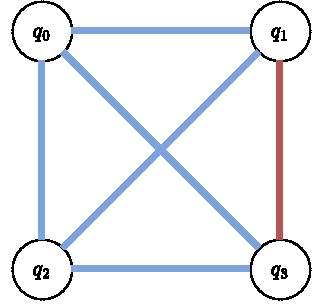
\includegraphics[width=0.46\textwidth]{./figure/class2_1.pdf} & 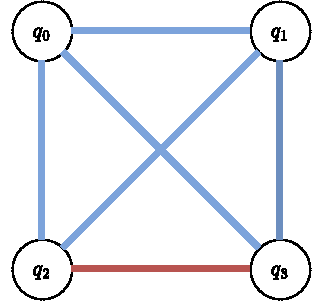
\includegraphics[width=0.46\textwidth]{./figure/class2_2.pdf}  \\
  \end{tabular}
\caption{caption}
\end{figure}
\paragraph{Class 2. } Only one interaction term is antiferromanetic. By using interchange operation, we can derive 6 elements as the same symmetry class.
For example, from the left one in the figure with coefficients $(1,1,1,1,-1,1)$, we can derive right one with coefficients $(1,1,1,1,1,-1)$ by using interchange operation on qubit $1$ and qubit $2$. 
The other models can be derived by applying one or multiple interchange operations. 

Class 3
\begin{table}[!h]
  \begin{tabular}{cccccc}
    \toprule\toprule
    $J_{01}$ & $J_{02}$ & $J_{03}$ & $J_{12}$ & $J_{13}$ & $J_{23}$ \\ 
    \midrule
    $1$ &$1$ &$1$ &$1$ &$-1$ &$-1$   \\
    $1$ &$1$ &$1$ &$-1$ &$1$ &$-1$   \\
    $1$ &$1$ &$1$ &$-1$ &$-1$ &$1$   \\
    $1$ &$1$ &$-1$ &$1$ &$1$ &$-1$   \\
    $1$ &$1$ &$-1$ &$1$ &$-1$ &$1$   \\
    $1$ &$-1$ &$1$ &$1$ &$1$ &$-1$   \\
    $1$ &$-1$ &$1$ &$-1$ &$1$ &$1$   \\
    $1$ &$-1$ &$-1$ &$1$ &$1$ &$1$   \\
    $-1$ &$1$ &$1$ &$1$ &$-1$ &$1$   \\
    $-1$ &$1$ &$1$ &$-1$ &$1$ &$1$   \\
    $-1$ &$1$ &$-1$ &$1$ &$1$ &$1$   \\
    $-1$ &$-1$ &$1$ &$1$ &$1$ &$1$   \\
    \bottomrule
    \caption{Example LaTeX Table} 
    \label{tab:example3}
  \end{tabular}
\end{table}

\begin{figure}[!h]
  \begin{tabular}{cc}
    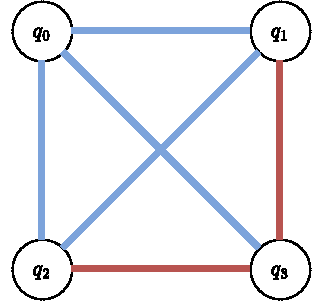
\includegraphics[width=0.46\textwidth]{./figure/class3_1.pdf} & 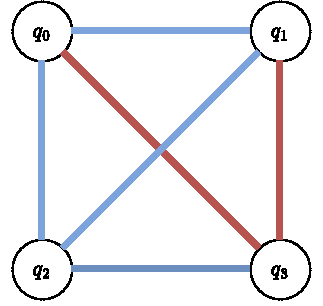
\includegraphics[width=0.46\textwidth]{./figure/class3_2.pdf}  \\
  \end{tabular}
\caption{caption}
\end{figure}
\paragraph{Class 3. } Two interaction terms are antiferromanetic.
As shown in the figure, one qubit has two antiferromanetic interaction.  By using interchange operation, we can derive 12 elements as the same symmetry class.
For example, from the left one in the figure with coefficients $(1,1,1,1,-1,-1)$, we can derive right one with coefficients $(1,1,-1,1,-1,1)$ by using interchange operation on qubit $0$ and qubit $2$. 
The other models can be derived by applying one or multiple interchange operations. 

Class 4
\begin{table}[!h]
  \begin{tabular}{cccccc}
    \toprule\toprule
    $J_{01}$ & $J_{02}$ & $J_{03}$ & $J_{12}$ & $J_{13}$ & $J_{23}$ \\ 
    \midrule
    $1$ &$1$ &$1$ &$-1$ &$-1$ &$-1$   \\
    $1$ &$-1$ &$-1$ &$1$ &$1$ &$-1$   \\
    $-1$ &$1$ &$-1$ &$1$ &$-1$ &$1$   \\
    $-1$ &$-1$ &$1$ &$-1$ &$1$ &$1$   \\
    \bottomrule
    \caption{Example LaTeX Table} 
    \label{tab:example4}
  \end{tabular}
\end{table}

\begin{figure}[!h]
  \begin{tabular}{cc}
    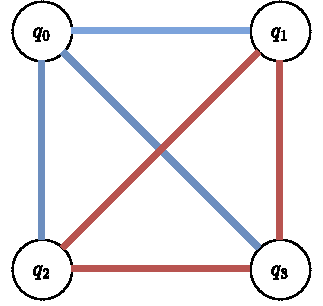
\includegraphics[width=0.46\textwidth]{./figure/class4_1.pdf} & 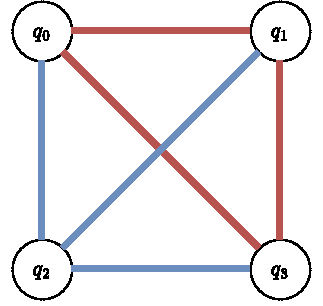
\includegraphics[width=0.46\textwidth]{./figure/class4_2.pdf}  \\
  \end{tabular}
\caption{caption}
\end{figure}
\paragraph{Class 3. } Three interaction terms are antiferromanetic.
As shown in the figure, three qubits have two antiferromanetic interactions while the remaining qubit has only ferromagnetic interaction. 
By using interchange operation, we can derive 4 elements as the same symmetry class.
For example, from the left one in the figure with coefficients $(1,1,1,-1,-1,-1)$, we can derive right one with coefficients $(-1,1,-1,1,-1,1)$ by using interchange operation on qubit $0$ and qubit $2$. 
The other models can be derived by applying one or multiple interchange operations. 

Class 5
\begin{table}[!h]
  \begin{tabular}{cccccc}
    \toprule\toprule
    $J_{01}$ & $J_{02}$ & $J_{03}$ & $J_{12}$ & $J_{13}$ & $J_{23}$ \\ 
    \midrule
    $1$ &$1$ &$-1$ &$1$ &$-1$ &$-1$   \\
    $1$ &$-1$ &$1$ &$-1$ &$1$ &$-1$   \\
    $-1$ &$1$ &$1$ &$-1$ &$-1$ &$1$   \\
    $-1$ &$-1$ &$-1$ &$1$ &$1$ &$1$   \\
    \bottomrule
    \caption{Example LaTeX Table} 
    \label{tab:example5}
  \end{tabular}
\end{table}
\begin{figure}[!h]
  \begin{tabular}{cc}
    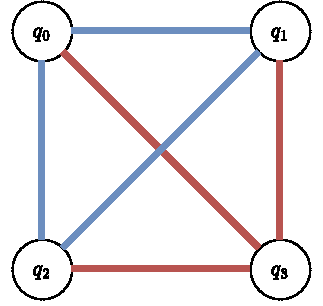
\includegraphics[width=0.46\textwidth]{./figure/class5_1.pdf} & 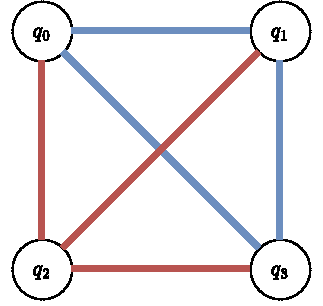
\includegraphics[width=0.46\textwidth]{./figure/class5_2.pdf}  \\
  \end{tabular}
\caption{caption}
\end{figure}
\paragraph{Class 5. } Three interaction terms are antiferromanetic.
As shown in the figure, one qubit has only antiferromanetic interactions. 
By using interchange operation, we can derive 4 elements as the same symmetry class.
For example, from the left one in the figure with coefficients $(1,1,-1,1,-1,-1)$, we can derive right one with coefficients $(1,-1,1,1,-1,-1)$ by using interchange operation on qubit $2$ and qubit $3$. 
The other models can be derived by applying one or multiple interchange operations. 


Class 6
\begin{table}[!h]
  \begin{tabular}{cccccc}
    \toprule\toprule
    $J_{01}$ & $J_{02}$ & $J_{03}$ & $J_{12}$ & $J_{13}$ & $J_{23}$ \\ 
    \midrule
    $1$ &$1$ &$-1$ &$-1$ &$1$ &$1$   \\
    $1$ &$-1$ &$1$ &$1$ &$-1$ &$1$   \\
    $-1$ &$1$ &$1$ &$1$ &$1$ &$-1$   \\
    \bottomrule
    \caption{Example LaTeX Table} 
    \label{tab:example6}
  \end{tabular}
\end{table}

\begin{figure}[!h]
  \begin{tabular}{cc}
    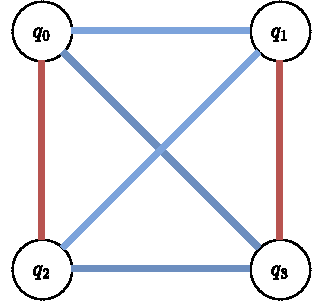
\includegraphics[width=0.46\textwidth]{./figure/class6_1.pdf} & 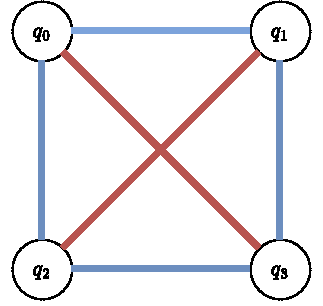
\includegraphics[width=0.46\textwidth]{./figure/class6_2.pdf}  \\
  \end{tabular}
\caption{caption}
\end{figure}
\paragraph{Class 6. } Two interaction terms are antiferromanetic.
As shown in the figure, all qubit has only one antiferromanetic interaction unlike class 2 symmetry group that one qubit has two antiferromanetic interaction. 
By using interchange operation, we can derive 3 elements as the same symmetry class.
For example, from the left one in the figure with coefficients $(1,-1,1,1,-1,1)$, we can derive right one with coefficients $(1,1,-1,-1,1,1)$ by using interchange operation on qubit $0$ and qubit $1$. 
The other model can be derived by applying one or multiple interchange operations. 

Class 7
\begin{table}[!h]
  \begin{tabular}{cccccc}
    \toprule\toprule
    $J_{01}$ & $J_{02}$ & $J_{03}$ & $J_{12}$ & $J_{13}$ & $J_{23}$ \\ 
    \midrule
    $1$ &$1$ &$-1$ &$-1$ &$1$ &$-1$   \\
    $1$ &$1$ &$-1$ &$-1$ &$-1$ &$1$   \\
    $1$ &$-1$ &$1$ &$1$ &$-1$ &$-1$   \\
    $1$ &$-1$ &$1$ &$-1$ &$-1$ &$1$   \\
    $1$ &$-1$ &$-1$ &$1$ &$-1$ &$1$   \\
    $1$ &$-1$ &$-1$ &$-1$ &$1$ &$1$   \\
    $-1$ &$1$ &$1$ &$1$ &$-1$ &$-1$   \\
    $-1$ &$1$ &$1$ &$-1$ &$1$ &$-1$   \\
    $-1$ &$1$ &$-1$ &$1$ &$1$ &$-1$   \\
    $-1$ &$1$ &$-1$ &$-1$ &$1$ &$1$   \\
    $-1$ &$-1$ &$1$ &$1$ &$1$ &$-1$   \\
    $-1$ &$-1$ &$1$ &$1$ &$-1$ &$1$   \\
    \bottomrule
    \caption{Example LaTeX Table} 
    \label{tab:example7}
  \end{tabular}
\end{table}

\begin{figure}[!h]
  \begin{tabular}{cc}
    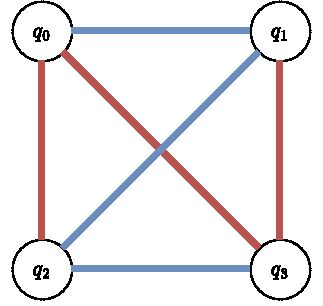
\includegraphics[width=0.46\textwidth]{./figure/class7_1.pdf} & 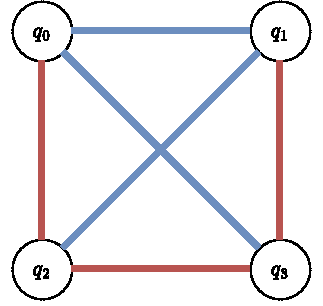
\includegraphics[width=0.46\textwidth]{./figure/class7_2.pdf}  \\
  \end{tabular}
\caption{caption}
\end{figure}
\paragraph{Class 7. } Three interaction terms are antiferromanetic.
As shown in the figure, each qubit has one or two antiferromanetic interactions. 
In this case, this symmetry class also pocesses sign-flip symmetry. 
After the sign flip operation, the Hamiltonian is still in the same class. 
By using interchange operation and sign flip operation, we can derive 12 elements as the same symmetry class.
For example, from the left one in the figure with coefficients $(1,-1,-1,1,-1,1)$, we can derive right one with coefficients $(1,-1,1,1,-1,-1)$ by using interchange operation on qubit $0$ and qubit $2$. 
The other model can be derived by applying one or multiple interchange operations and sign flip operation. 

Class 8
\begin{table}[!h]
  \begin{tabular}{cccccc}
    \toprule\toprule
    $J_{01}$ & $J_{02}$ & $J_{03}$ & $J_{12}$ & $J_{13}$ & $J_{23}$ \\ 
    \midrule
    $1$ &$1$ &$-1$ &$-1$ &$-1$ &$-1$   \\
    $1$ &$-1$ &$1$ &$-1$ &$-1$ &$-1$   \\
    $1$ &$-1$ &$-1$ &$1$ &$-1$ &$-1$   \\
    $1$ &$-1$ &$-1$ &$-1$ &$1$ &$-1$   \\
    $-1$ &$1$ &$1$ &$-1$ &$-1$ &$-1$   \\
    $-1$ &$1$ &$-1$ &$1$ &$-1$ &$-1$   \\
    $-1$ &$1$ &$-1$ &$-1$ &$-1$ &$1$   \\
    $-1$ &$-1$ &$1$ &$-1$ &$1$ &$-1$   \\
    $-1$ &$-1$ &$1$ &$-1$ &$-1$ &$1$   \\
    $-1$ &$-1$ &$-1$ &$1$ &$1$ &$-1$   \\
    $-1$ &$-1$ &$-1$ &$1$ &$-1$ &$1$   \\
    $-1$ &$-1$ &$-1$ &$-1$ &$1$ &$1$   \\
    \bottomrule
    \caption{Example LaTeX Table} 
    \label{tab:example8}
  \end{tabular}
\end{table}

\begin{figure}[!h]
  \begin{tabular}{cc}
    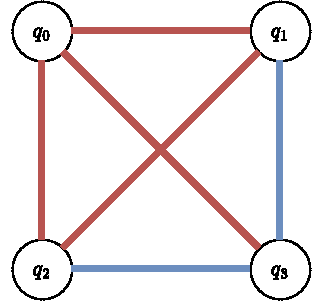
\includegraphics[width=0.46\textwidth]{./figure/class8_1.pdf} & 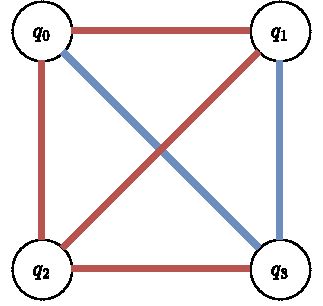
\includegraphics[width=0.46\textwidth]{./figure/class8_2.pdf}  \\
  \end{tabular}
\caption{caption}
\end{figure}
\paragraph{Class 8. } 
From now on, it is convenient to focus on ferromagnetic interaction.
Two interaction terms are ferromagnetic.
As shown in the figure, one qubit has two antiferromanetic interaction. 
By using interchange operation, we can derive 12 elements as the same symmetry class. 
For example, from the left one in the figure with coefficients $(-1,-1,-1,-1,1,1)$, we can derive right one with coefficients $(-1,-1,1,-1,1,-1)$ by using interchange operation on qubit $0$ and qubit $2$. 
The other models can be derived by applying one or multiple interchange operations. 
Note that this symmetry class can also derived by sign flip operation on symmetry class 3.


Class 9
\begin{table}[!h]
  \begin{tabular}{cccccc}
    \toprule\toprule
    $J_{01}$ & $J_{02}$ & $J_{03}$ & $J_{12}$ & $J_{13}$ & $J_{23}$ \\ 
    \midrule
    $1$ &$-1$ &$-1$ &$-1$ &$-1$ &$1$   \\
    $-1$ &$1$ &$-1$ &$-1$ &$1$ &$-1$   \\
    $-1$ &$-1$ &$1$ &$1$ &$-1$ &$-1$   \\
    \bottomrule
    \caption{Example LaTeX Table} 
    \label{tab:example9}
  \end{tabular}
\end{table}

\begin{figure}[!h]
  \begin{tabular}{cc}
    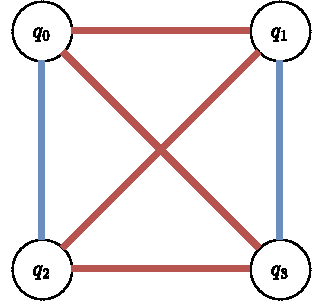
\includegraphics[width=0.46\textwidth]{./figure/class9_1.pdf} & 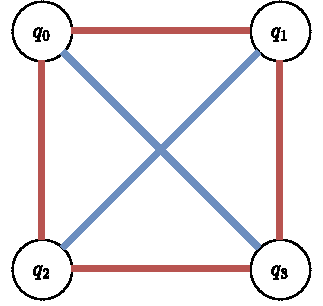
\includegraphics[width=0.46\textwidth]{./figure/class9_2.pdf}  \\
  \end{tabular}
\caption{caption}
\end{figure}
\paragraph{Class 9. } 
Two interaction terms are ferromagnetic.
As shown in the figure, each qubit has only one antiferromanetic interaction. 
By using interchange operation, we can derive 3 elements as the same symmetry class. 
For example, from the left one in the figure with coefficients $(-1,1,-1,-1,1,-1)$, we can derive right one with coefficients $(-1,-1,1,1,-1,-1)$ by using interchange operation on qubit $0$ and qubit $1$. 
The other model can be derived by applying one or multiple interchange operations. 
Note that this symmetry class can also derived by sign flip operation on symmetry class 6.


Class 10
\begin{table}[!h]
  \begin{tabular}{cccccc}
    \toprule\toprule
    $J_{01}$ & $J_{02}$ & $J_{03}$ & $J_{12}$ & $J_{13}$ & $J_{23}$ \\ 
    \midrule
    $1$ &$-1$ &$-1$ &$-1$ &$-1$ &$-1$   \\
    $-1$ &$1$ &$-1$ &$-1$ &$-1$ &$-1$   \\
    $-1$ &$-1$ &$1$ &$-1$ &$-1$ &$-1$   \\
    $-1$ &$-1$ &$-1$ &$1$ &$-1$ &$-1$   \\
    $-1$ &$-1$ &$-1$ &$-1$ &$1$ &$-1$   \\
    $-1$ &$-1$ &$-1$ &$-1$ &$-1$ &$1$   \\
    \bottomrule
    \caption{Example LaTeX Table} 
    \label{tab:example10}
  \end{tabular}
\end{table}

\begin{figure}[!h]
  \begin{tabular}{cc}
    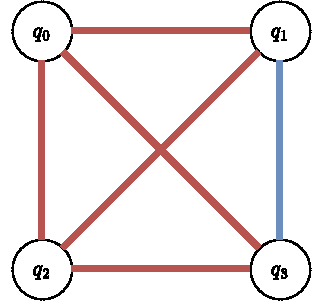
\includegraphics[width=0.46\textwidth]{./figure/class10_1.pdf} & 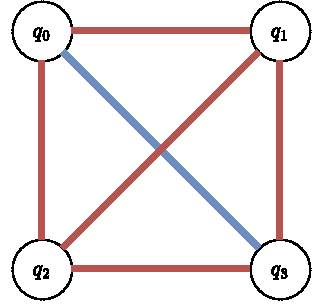
\includegraphics[width=0.46\textwidth]{./figure/class10_2.pdf}  \\
  \end{tabular}
\caption{caption}
\end{figure}
\paragraph{Class 10. } 
Only one interaction term is ferromagnetic.
By using interchange operation, we can derive 6 elements as the same symmetry class. 
For example, from the left one in the figure with coefficients $(-1,-1,-1,-1,1,-1)$, we can derive right one with coefficients $(-1,-1,1,-1,-1,-1)$ by using interchange operation on qubit $0$ and qubit $1$. 
The other model can be derived by applying one or multiple interchange operations. 
Note that this symmetry class can also derived by sign flip operation on symmetry class 2.

Class 11
\begin{table}[!h]
  \begin{tabular}{cccccc}
    \toprule\toprule
    $J_{01}$ & $J_{02}$ & $J_{03}$ & $J_{12}$ & $J_{13}$ & $J_{23}$ \\ 
    \midrule
    $-1$ &$-1$ &$-1$ &$-1$ &$-1$ &$-1$   \\
    \bottomrule
    \caption{Example LaTeX Table} 
    \label{tab:example11}
  \end{tabular}
\end{table}

\begin{figure}[!h]
  \centering
  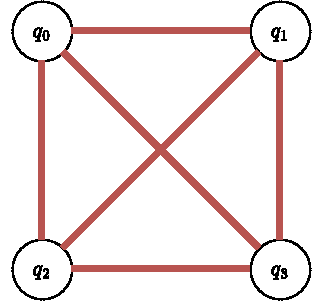
\includegraphics[width=0.5\textwidth]{./figure/class11.pdf}
  \caption{caption}
\end{figure}
\paragraph{Class 11. } 
The whole interactions are antiferromagnetic. There is no other possible element even by using interchange interaction. 
This symmetry class can be derived from sign flip operation on symmetry class 1.

\subsection*{What is the eigenspectrum of each symmetry class?}

\begin{figure}
  \begin{tabular}{ccc}
    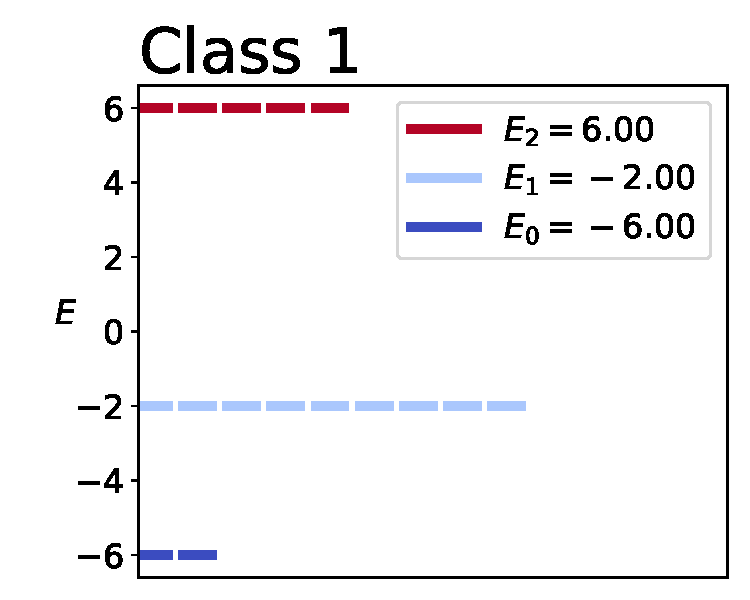
\includegraphics[width=0.3\textwidth]{./figure/class_1.pdf} & 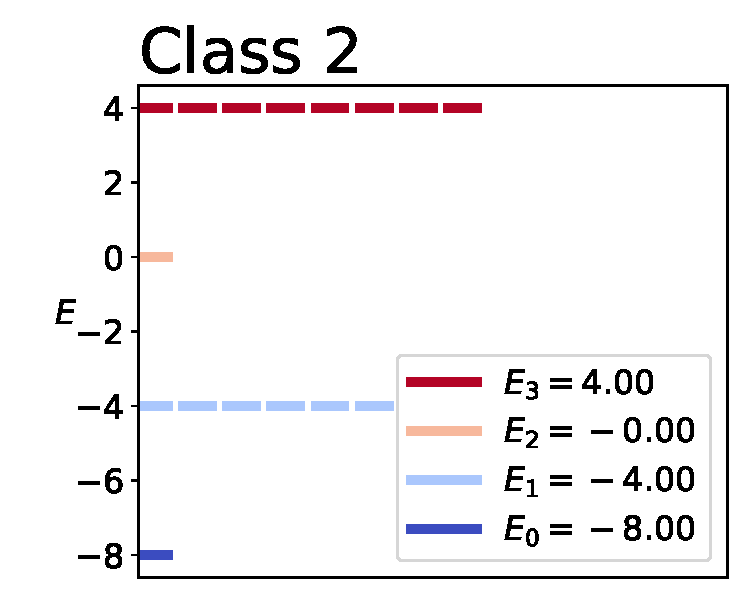
\includegraphics[width=0.3\textwidth]{./figure/class_2.pdf} & 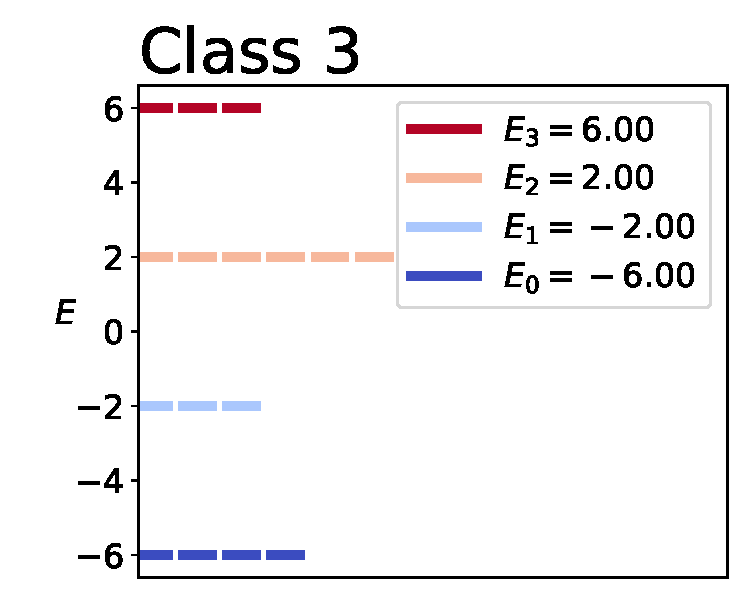
\includegraphics[width=0.3\textwidth]{./figure/class_3.pdf} \\
    %(a) & (b) & (c) \\
    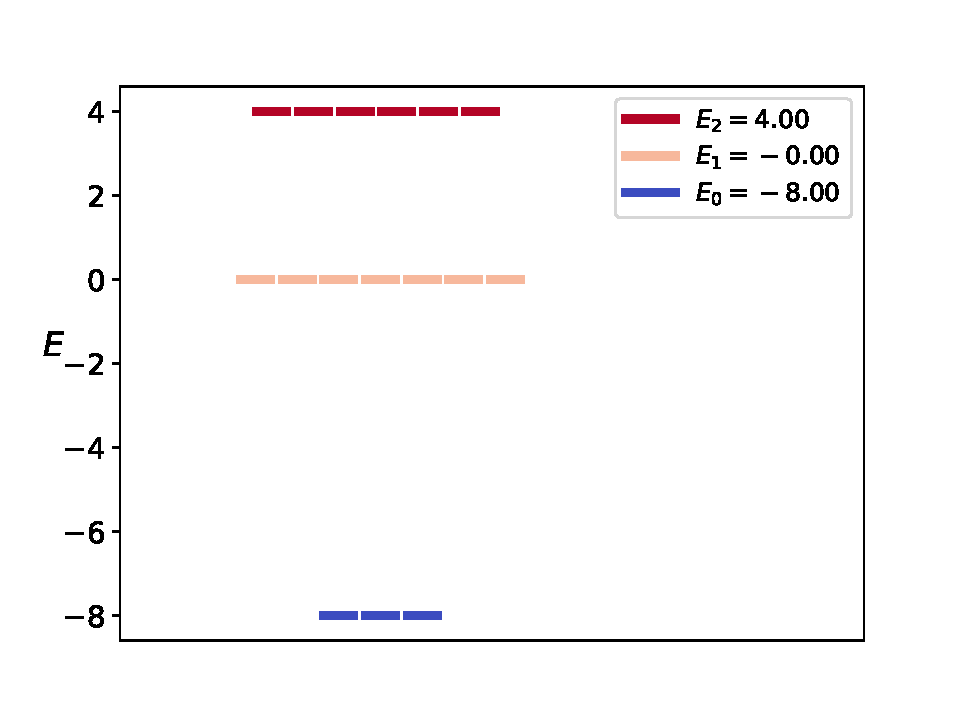
\includegraphics[width=0.3\textwidth]{./figure/class_4.pdf} & 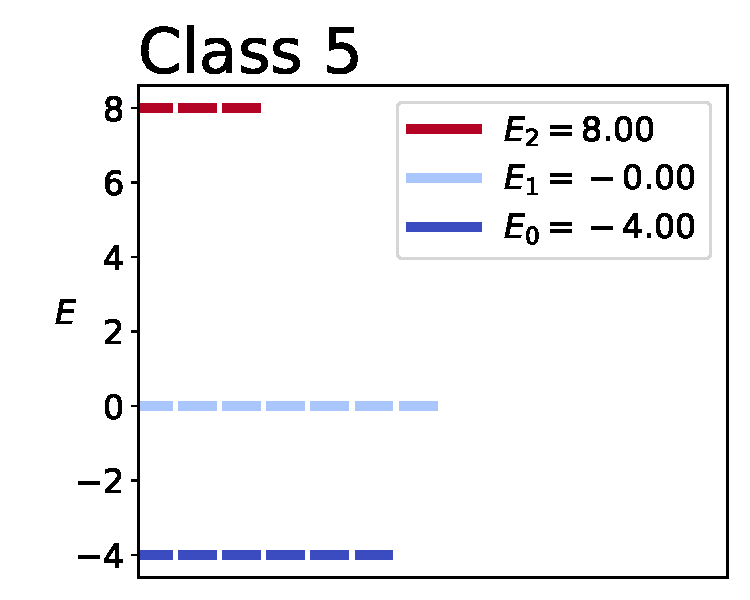
\includegraphics[width=0.3\textwidth]{./figure/class_5.pdf} & 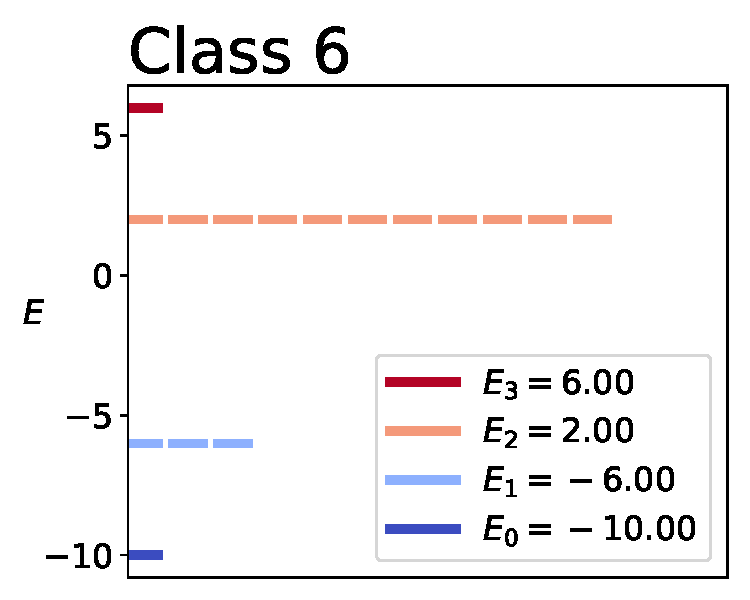
\includegraphics[width=0.3\textwidth]{./figure/class_6.pdf} \\
    %(d) & (e) & (f) \\
    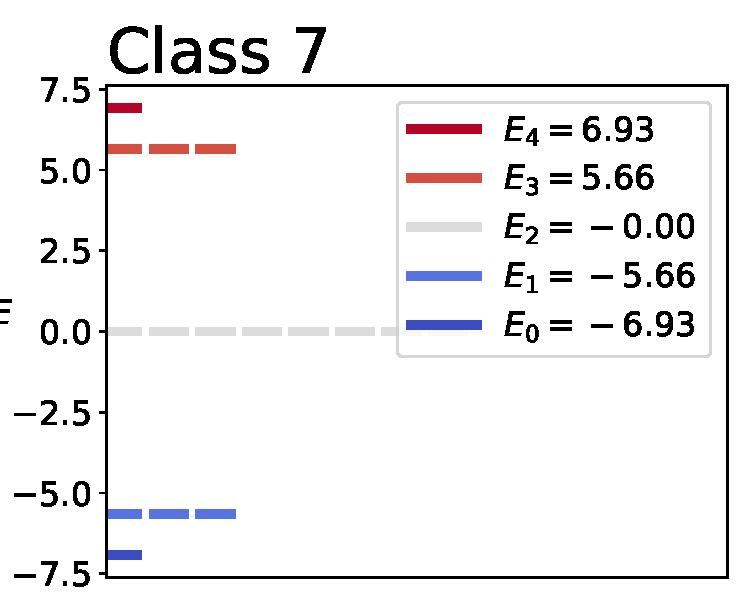
\includegraphics[width=0.3\textwidth]{./figure/class_7.pdf} & 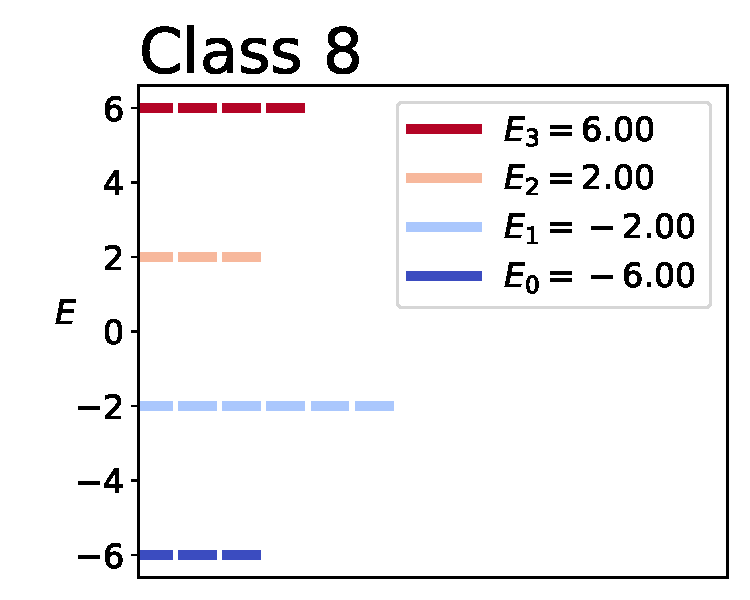
\includegraphics[width=0.3\textwidth]{./figure/class_8.pdf} & 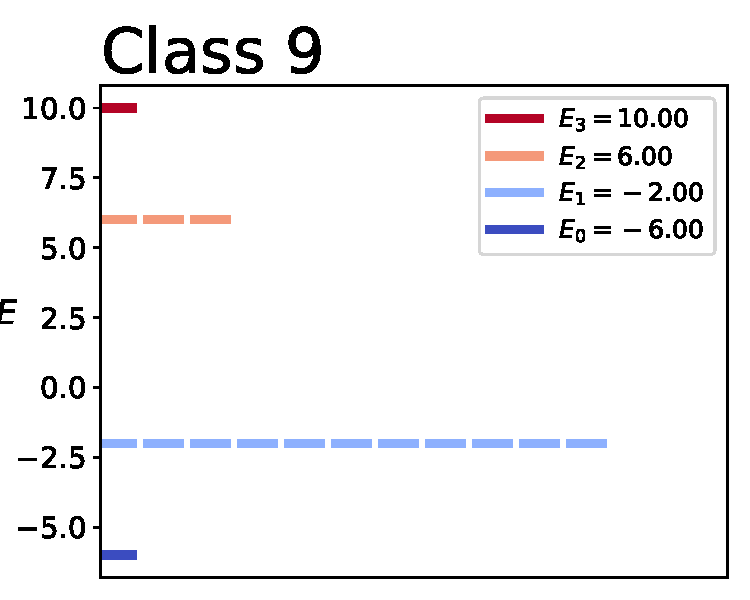
\includegraphics[width=0.3\textwidth]{./figure/class_9.pdf} \\
    %(g) & (h) & (i) \\
    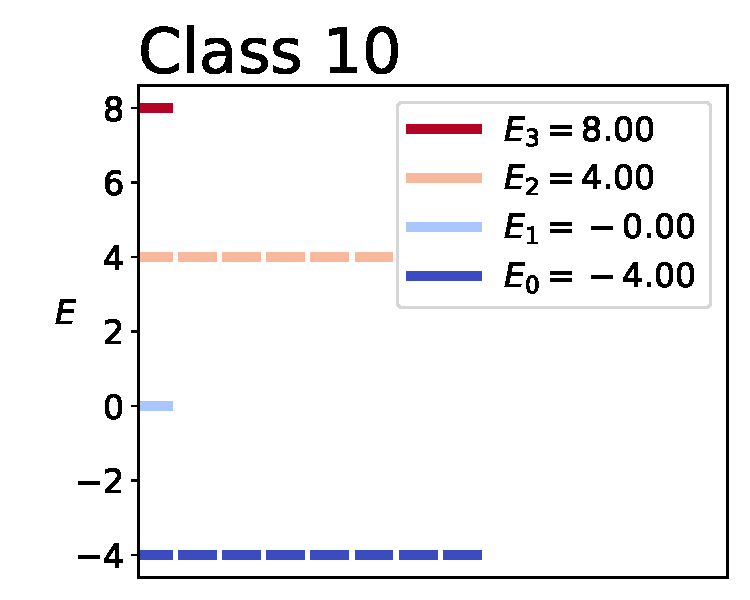
\includegraphics[width=0.3\textwidth]{./figure/class_10.pdf}& 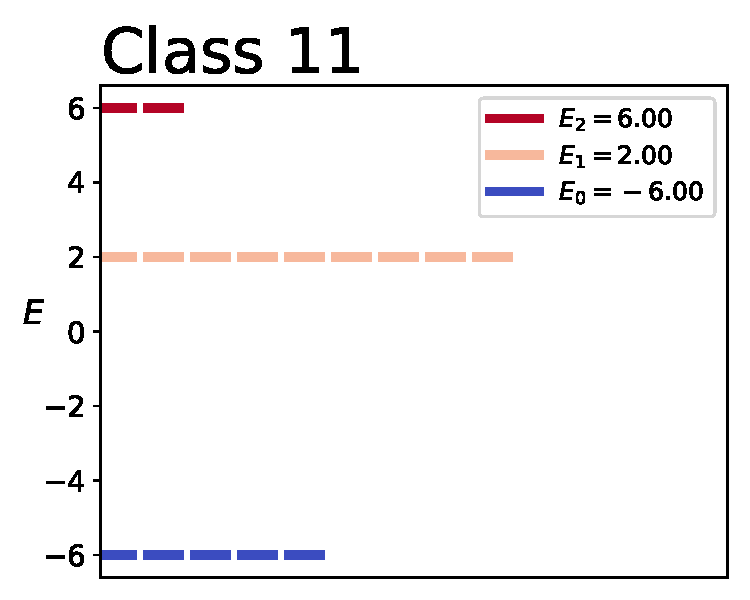
\includegraphics[width=0.3\textwidth]{./figure/class_11.pdf}& \\
    %(j) & (k) &  
  \end{tabular}
\caption{caption}
\end{figure}

\subsection*{Do any of the symmetry classes have an eigenspectrum that is sign invariant? In other words, if you change the sign of each eigenvalue, does the overall set of eigenvalues remain unchanged?}

As shown in Figure , the eigenspectrum of class 7 has sign flip invariance. 
It is because the Hamiltonian of class 7 is still in the class 7 even after sign flip operation. 

\section*{Part 2 : Adiabatic evolution to the ground state}

\subsection*{Plot the eigenspectra as a function of $s$ for each symmetry class.}
Class 1 
\begin{figure}[!h]
  \begin{tabular}{ccc}
    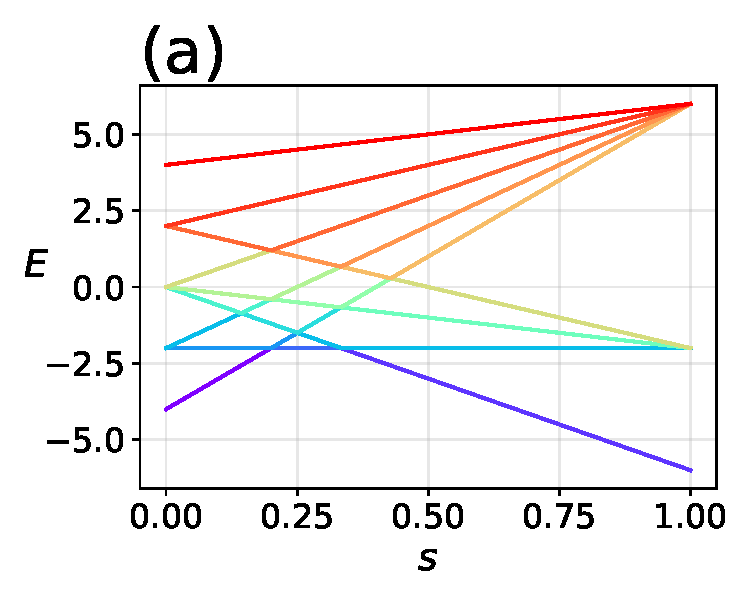
\includegraphics[width=0.3\textwidth]{./figure/Eigenspectrum_class_1.pdf} & 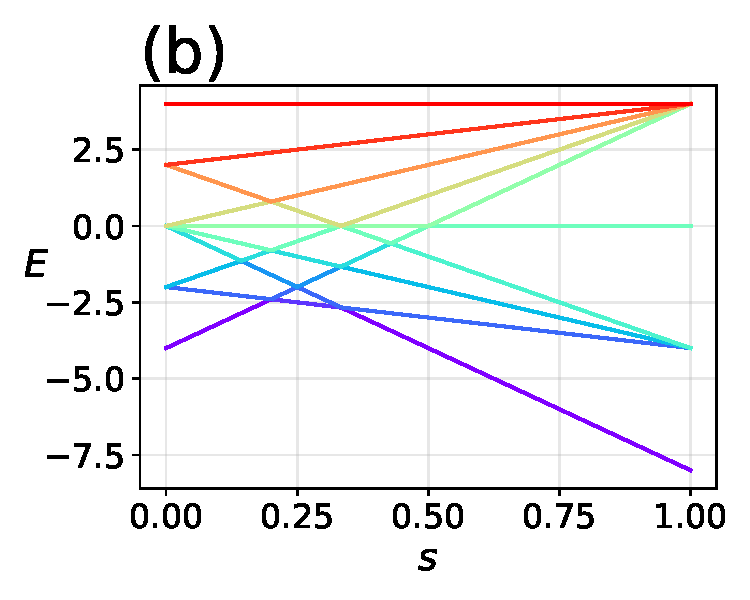
\includegraphics[width=0.3\textwidth]{./figure/Eigenspectrum_class_2.pdf} & 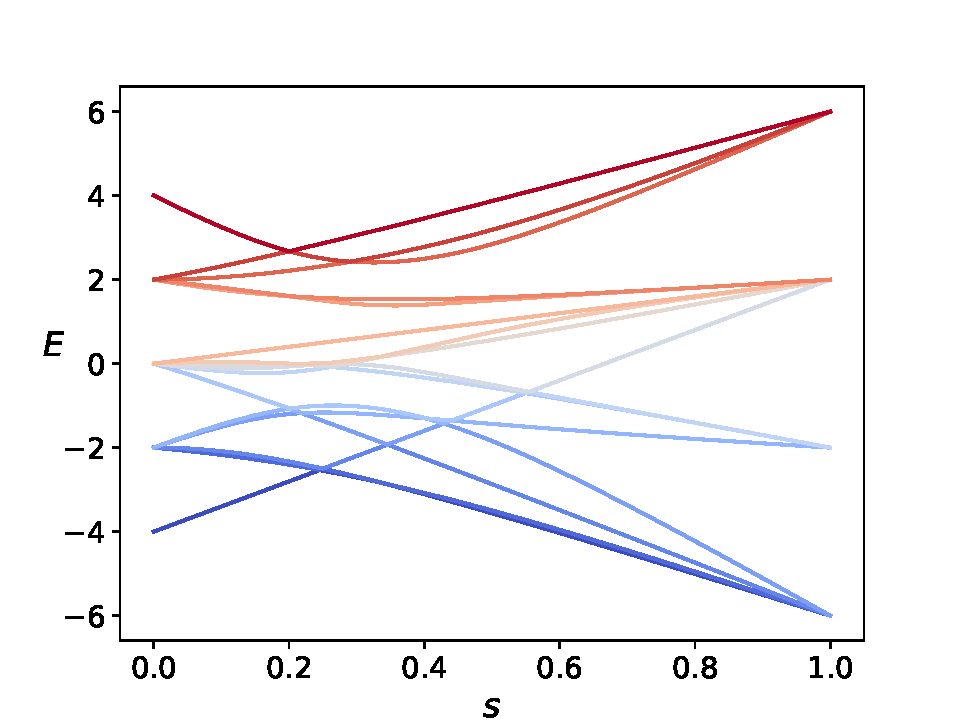
\includegraphics[width=0.3\textwidth]{./figure/Eigenspectrum_class_3.pdf} \\
    %(a) & (b) & (c) \\
    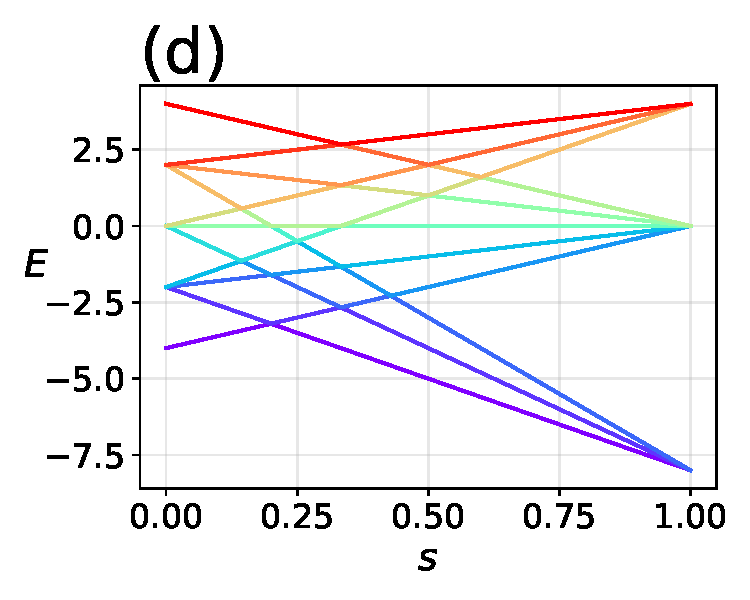
\includegraphics[width=0.3\textwidth]{./figure/Eigenspectrum_class_4.pdf} & 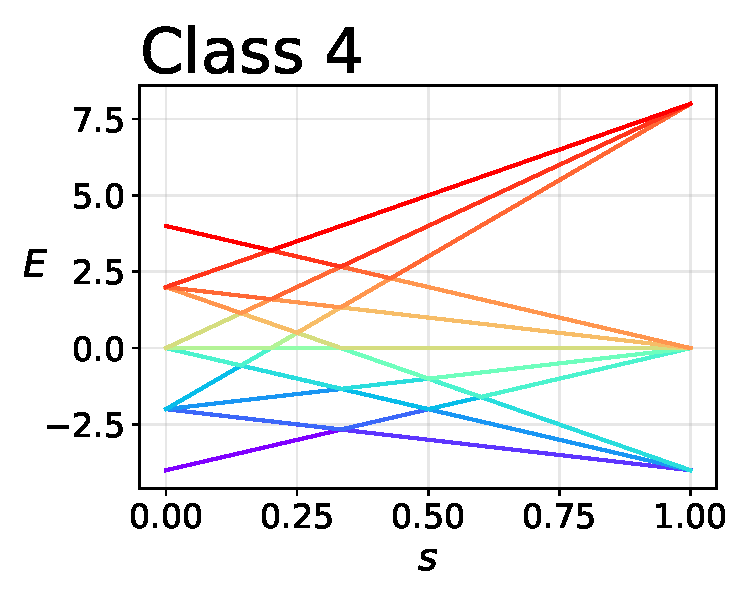
\includegraphics[width=0.3\textwidth]{./figure/Eigenspectrum_class_5.pdf} & 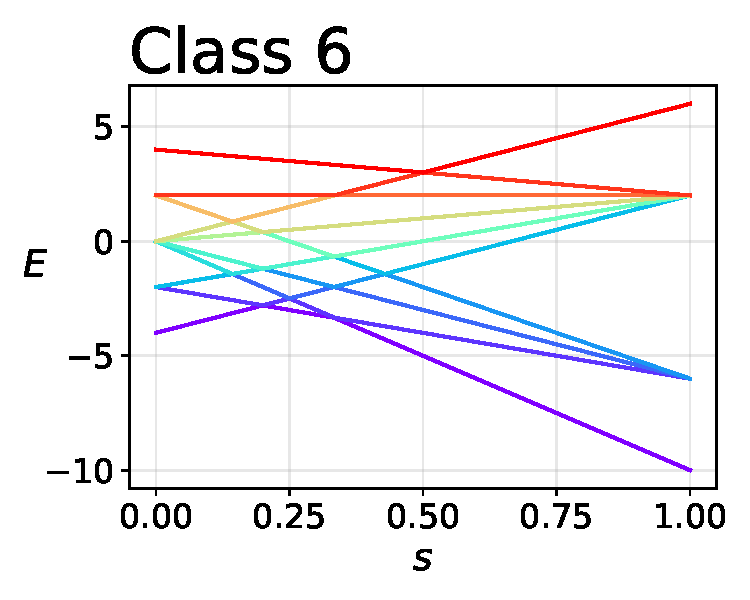
\includegraphics[width=0.3\textwidth]{./figure/Eigenspectrum_class_6.pdf} \\
    %(d) & (e) & (f) \\
    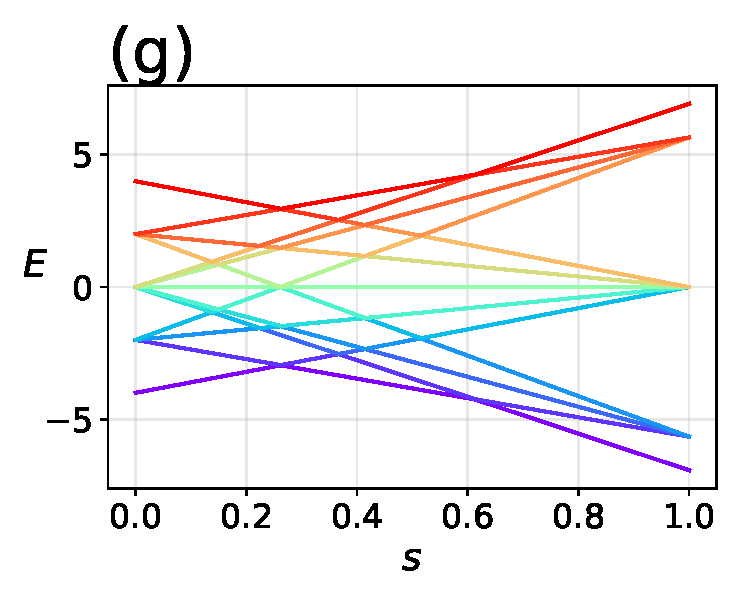
\includegraphics[width=0.3\textwidth]{./figure/Eigenspectrum_class_7.pdf} & 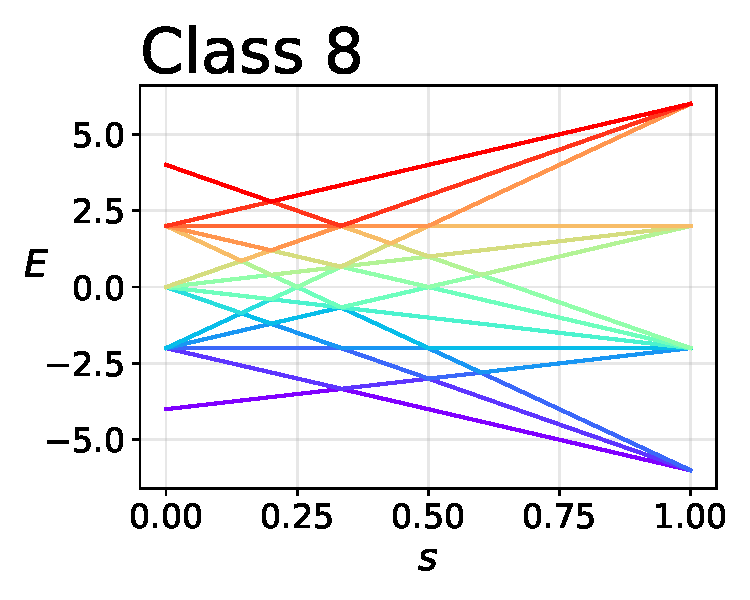
\includegraphics[width=0.3\textwidth]{./figure/Eigenspectrum_class_8.pdf} & 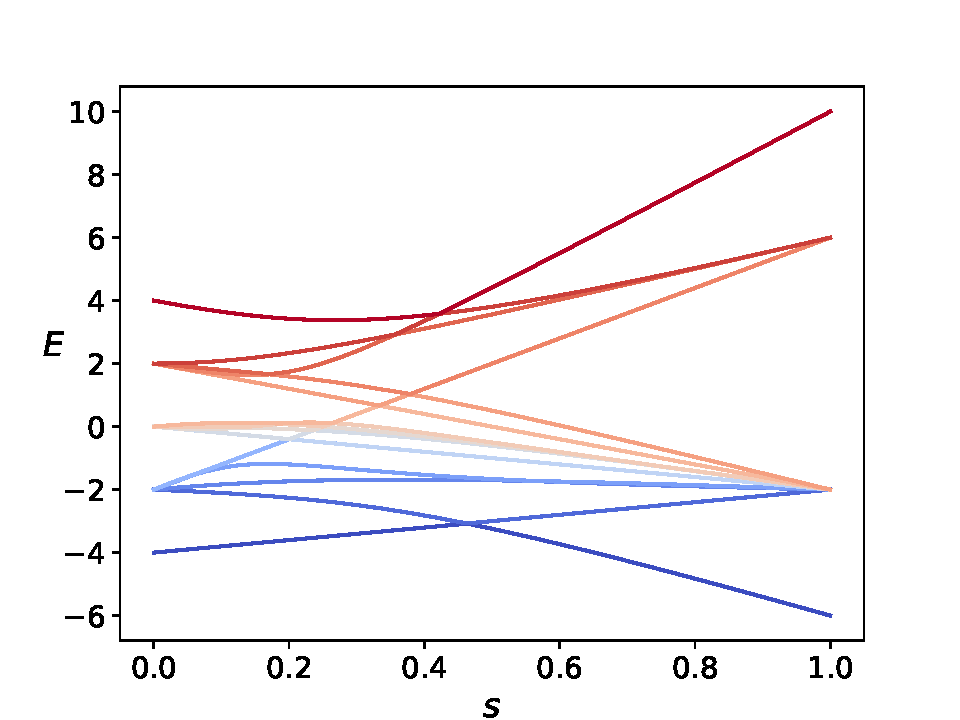
\includegraphics[width=0.3\textwidth]{./figure/Eigenspectrum_class_9.pdf} \\
    %(g) & (h) & (i) \\
    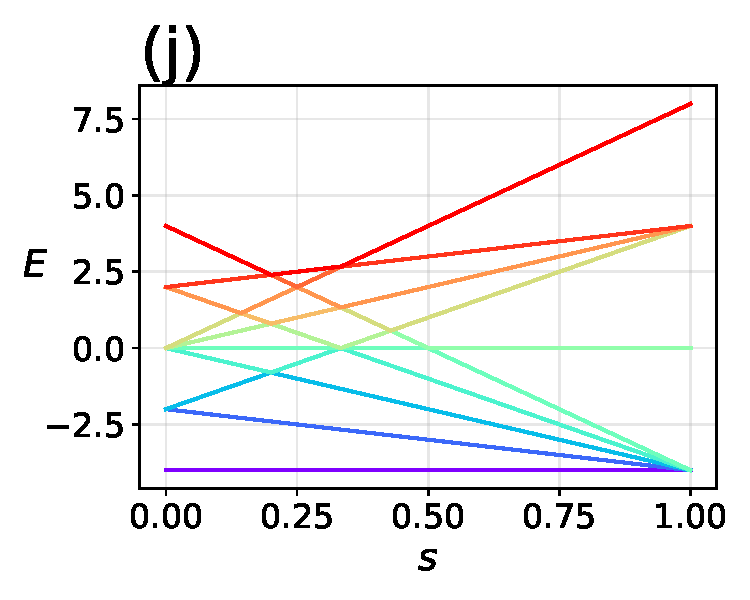
\includegraphics[width=0.3\textwidth]{./figure/Eigenspectrum_class_10.pdf}& 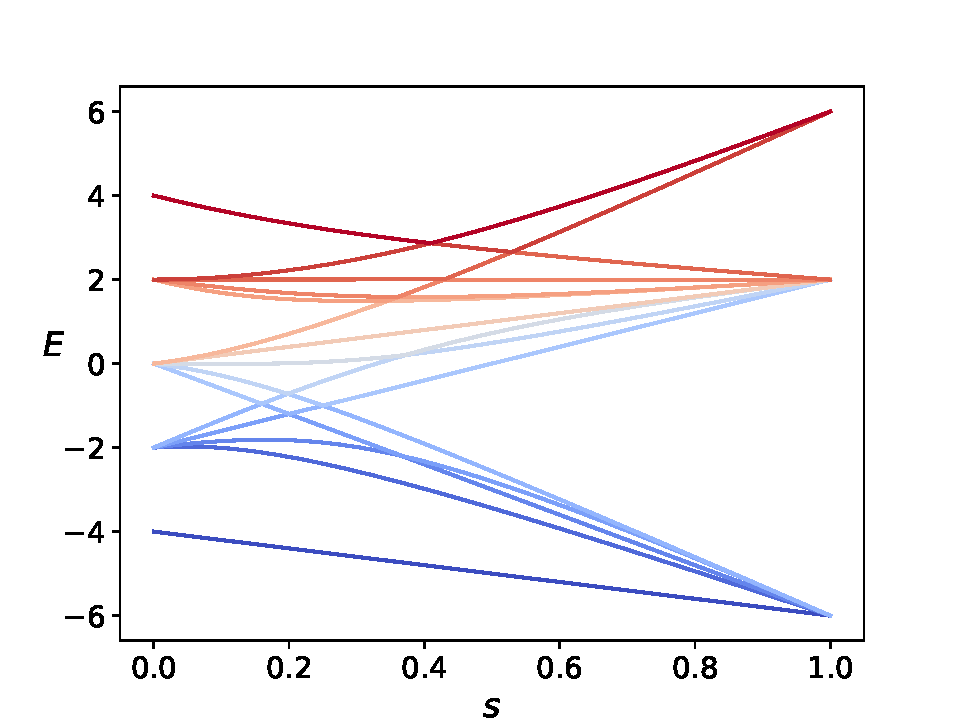
\includegraphics[width=0.3\textwidth]{./figure/Eigenspectrum_class_11.pdf}& \\
    %(j) & (k) &  
  \end{tabular}
\caption{caption}
\end{figure}

\subsection*{Plot the eigenspectrum for $H_{sg}$ as a function of $s$.}
\begin{figure}[!h]
  \centering
  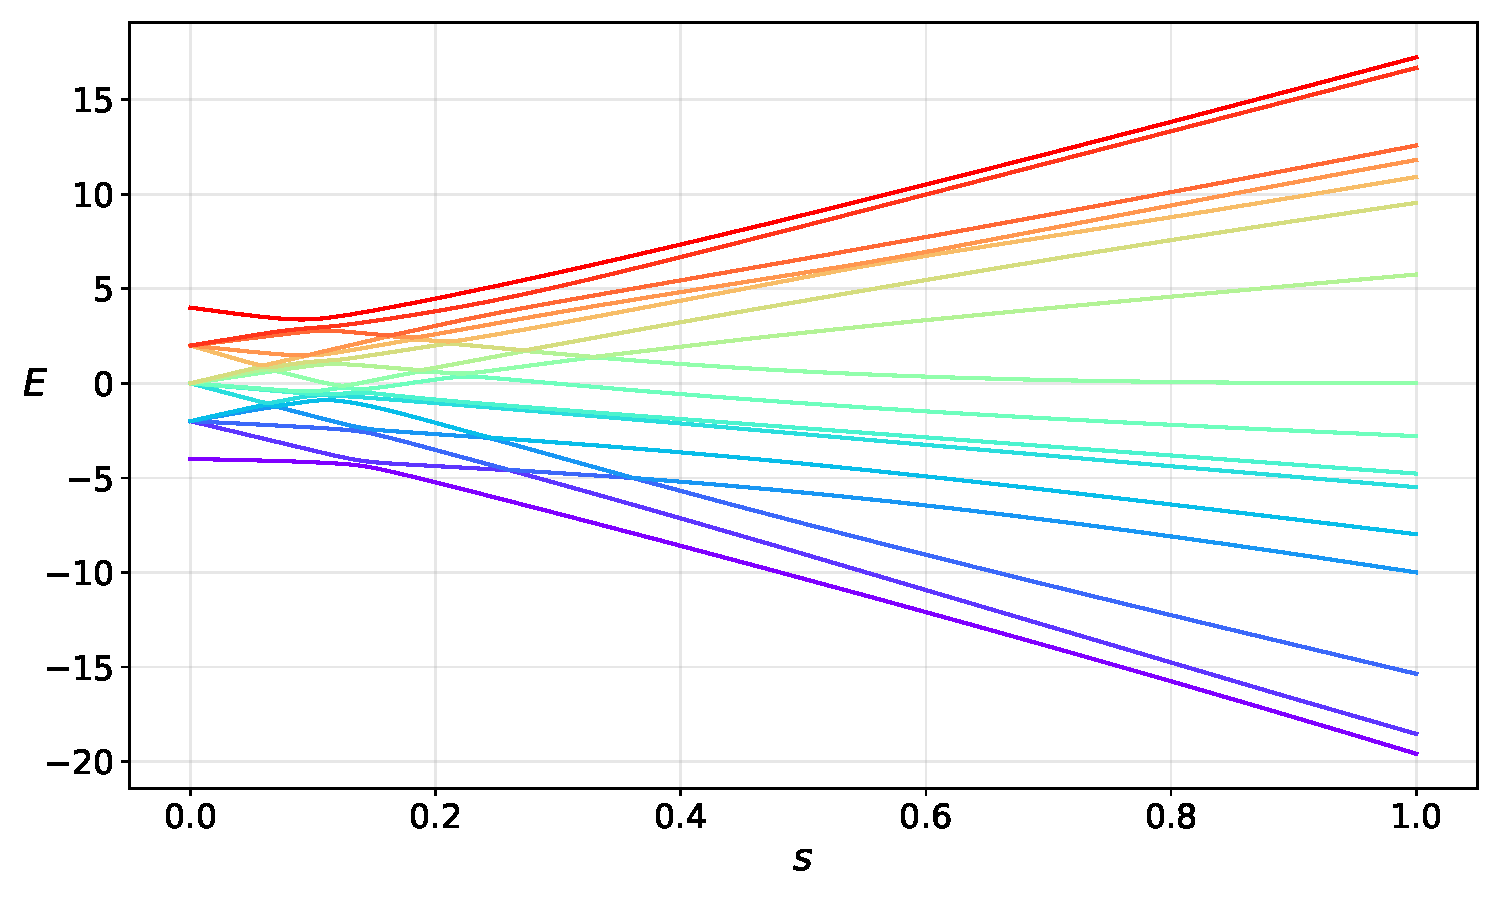
\includegraphics[width=0.9\textwidth]{./figure/Eigenspectrum_Heisenberg_sg.pdf}
  \caption{}
\end{figure}

\subsection*{Write a program to carry out adiabatic evolution, starting from the pure mixer Hamiltonian and ending with $H_{sg}$. Two parameters govern this program: the time $\tau$ over which the adiabatic evolution takes place and the number of time steps $N$.}
\begin{minted}[bgcolor=bg,
  frame=lines,
  framesep=2mm]{python}
def AdiabaticEvolution(self, tau, N):
  time_step = np.linspace(0, tau, N)
  dt = time_step[1] - time_step[0]
  
  ground_state = np.ones(2**self.num_qubits)
                /np.sqrt(2**self.num_qubits)
  for t in time_step:
    H = self.Propagator(t/tau)
    propagator = scipy.linalg.expm(-1j*dt*H)
    ground_state = propagator @ ground_state
  
  return ground_state
\end{minted}

\subsection*{In order to match the target vector of sixteen probabilities by performing adiabatic evolution, what value do you need to use for $\tau$ and $N$? The exact target probabilities and the probabilities resulting from adiabatic evolution should match to three significant decimal digits.}
The required running time for adiabatic evolution is known to the eigenspectrum of $H_{s}$, in particular the energy gap, $\delta$,  between the two lowest enery eigenvalues. 
The time for adiabatic evolution must obey:
\begin{equation}
  \tau \gg \frac{\epsilon}{\triangle^{2}}
\end{equation}
where $\triangle = \min_{0\leq s \leq 1} (E_1 (s) - E_0 (s))$ and $\epsilon$ is the largest value of $H_{P} - H_{0}$. 
In our case, $\triangle \simeq 0.2666$ and $\epsilon \simeq 17.79$, then, we have $\tau \simeq 250.4$. 
Then, I tuned $\tau$ and the number of step $N$, which is determined by $dt$, I found that $tau=1000$ and $N=2000$ yield our desired result. 


\subsection*{List out the terms in $H_{sg}$ and $H_{m}$ and, for each term, provide the gate that arises when that term is exponentiated. You can use any gate in Qiskit's standard gate set. How many single-qubit gates are needed for each time step? How many two-qubit gates are needed for each time step?}
Heisenberg Spin Glass

\subsection*{Assess the circuit needed to carry out the adiabatic evolution. Roughly how many single-qubit gates and two-qubit gates would be required to achieve three-digit accuracy for the sixteen probabilities characterizing the ground state? Do you think this is practical?}
It seems that the adiabatic evolution is not that practical.

\section*{Part 3 : A simpler path to the ground state}

\subsection*{Build a numerical program as outlined above, which contains arbitrary angle parameters and qubit pairs for XY-mixers. Experiment with the XY-mixers to obtain angle parameters and qubit pairs that rotate the final state so that its probabilities match the ground state probabilities of $H_{sg}$. This problem can be solved using three XY-mixers.}
I used ansatz the state, initialized to $\ket{1110}$ first and three XY-mixer acting on qubit-0 and -1, qubit-0 and -2, and qubit-0 and -3. 
The following code performs the same operation:
\begin{minted}[bgcolor=bg,
  frame=lines,
  framesep=2mm]{python}
def ansatz(self, parameters):
  if len(self.index) != len(parameters):
    raise ValueError("Lengh should be matched")
  
  state = np.zeros(16, dtype=np.complex64)
  state[14] = 1

  operation = [self._XY_mixer(pair, parameter) 
                for pair, parameter 
                in zip(self.index, parameters)]
  for op in operation:
    state = op @ state

  return state
\end{minted}

\subsection*{Convert the numerical program into a quantum circuit. Verify that the output of this quantum circuit generates the correct probabilities for the ground state of $H_{sg}$.}
Noting that $\left[\sigma_x^{i}\sigma_x^{j}, \sigma_y^{i}\sigma_y^{j} \right] = 0$ the XY-mixer can be decomposed into $e^{-i\frac{\theta}{2} \left( \sigma_x^{i}\sigma_x^{j} + \sigma_y^{i}\sigma_y^{j}\right)} = e^{-i\frac{\theta}{2}  \sigma_x^{i}\sigma_x^{j}} e^{-i\frac{\theta}{2}  \sigma_y^{i}\sigma_y^{j}}$, that is, a combination of RXX gate and RYY gate.
Then, our quantum circuit can be implemented (i) apply X gate on qubit $1,2,3$, (ii) apply RXX and RYY gate on (0,1), (0,2), (0,3) qubits. 
This will yield a state that produces the similar signal distribution with the exact ground state. The code is implemented as:
\begin{minted}[bgcolor=bg,
  frame=lines,
  framesep=2mm]{python}
def circuit(self, parameters):
  qc = qiskit.QuantumCircuit(self.num_qubits)
  for i in range(1,self.num_qubits):
    qc.x(i)
  for pair, parameter in zip(self.index, parameters):
    qc.rxx(parameter, pair[0], pair[1])
    qc.ryy(parameter, pair[0], pair[1])

  return qc
\end{minted}

\subsection*{Check the phases of the non-zero components of the quantum circuit created in 3.b. Are they all real? If so, you can skip this step. Otherwise, find circuit elements that you can add to the end of your circuit so that all non-zero computational basis states have the same phase.}
The exact ground state has only real coefficients whose sign is $(+,+,+,-)$ in a order of $\ket{0111}, \ket{1011},\ket{1101},\ket{1110}$.
However, the circuit shown above generates a state whose coefficient of $ket{1110}$ is real while other coefficients are pure imaginary. 
\begin{align}
  e^{-i\frac{\theta_{3}}{2} \left( \sigma_x^{0}\sigma_x^{3} + \sigma_y^{0}\sigma_y^{3}\right)}
  e^{-i\frac{\theta_{2}}{2} \left( \sigma_x^{0}\sigma_x^{2} + \sigma_y^{0}\sigma_y^{2}\right)}
  e^{-i\frac{\theta_{1}}{2} \left( \sigma_x^{0}\sigma_x^{1} + \sigma_y^{0}\sigma_y^{1}\right)}
  \ket{1110} &= -i\cos\theta_{1}\cos\theta_{2}\sin\theta_{3}\ket{0111} +i\cos\theta_{1}\sin\theta_{2}\ket{1011} -i\sin\theta_{1} \ket{1101} - \cos\theta_{1}\cos\theta_{2}\cos\theta_{3}\ket{1110}
\end{align}
For convenience, let me denote it as a vector $(-i\cos\theta_{1}\cos\theta_{2}\sin\theta_{3}, i\cos\theta_{1}\sin\theta_{2}\ket{1011} -i\sin\theta_{1} , - \cos\theta_{1}\cos\theta_{2}\cos\theta_{3})$.
After applying RZ gate on qubit 0 with an angle $\frac{\pi}{2}$, to make imaginary terms to real.
Then next we should tune the sign of each term to be  $(+,+,+,-)$ or  $(-,-,-,+)$. 
Noting that a RZ gate with angle $\pi$ has effect that no sign change when the state of target qubit is 0, sign change otherwise. 
The solution is quite simple. If the sign of a term is differ from the one of $\ket{1110}$, there is not any required additional operations. 
Even, there is another $R_{z}(\pi)$ operation on the other qubit there is no other change on that sign relation. 
Therefore, if the sign of the coefficients of a basis whose $0$ state is on $i$ qubit is same with the one of $\ket{1110}$, apply $R_z{\pi}$ on qubit $i$. 
This will results in correct ground state. The full code implementation including using XY-mixer and phase adjustment is below:
\begin{minted}[bgcolor=bg,
  frame=lines,
  framesep=2mm]{python}
def circuit(self, parameters):
  qc = qiskit.QuantumCircuit(self.num_qubits)
  for i in range(1,self.num_qubits):
    qc.x(i)
  for pair, parameter in zip(self.index, parameters):
    qc.rxx(parameter, pair[0], pair[1])
    qc.ryy(parameter, pair[0], pair[1])

  qc.rz(np.pi/2, 0)
  temp = self.ansatz(parameters)[[7,11,13,14]]

  temp[0:3] *= (1j if temp[3] > 0 else -1j)
  temp = (temp > 0)
  for i in range(3):
    qc.rz(np.pi, 3-i) if temp[i] else None

  self.qc = qc

  return qc
\end{minted}

\subsection*{Use your quantum circuit to measure the expectation value of the ground state of $H_{sg}$ . You will have to repeat your circuit three times - once to measure in each of the X, Y and Z computational bases. Each term of $H_{sg}$ can be measured in one of the three computational bases. Sum the contributions from the three bases and confirm that the summed energy is equal to the ground state eigenvalue}

Trivially, the expectation value of the system Hamiltonian $H_{sg}$ is sum of the expectation value of its components. 
Here, I gonna propose a general methodology to extract expectation value of $\sigma_{z}^{i}$ and $\sigma_{z}^{i}\sigma_{z}^{j}$.
First, $\sigma_{z}^{i}$ can be decomposed into:
\begin{align}
  \sigma_{z}^{i} &= I_{2}^{\otimes 3-i} \otimes \sigma_{z} \otimes I_{2}^{\otimes i} \\
  &=  \left(\ketbra{0} + \ketbra{1}\right)^{\otimes 3-i} \otimes \left(\ketbra{0} - \ketbra{1}\right) \otimes \left(\ketbra{0} + \ketbra{1}\right)^{\otimes i} \\
\end{align}
where $I_2$ is $2\times 2$ idenity matrix.
Then the expectation value of $\sigma_{z}^{i}$ for a given state is:
\begin{align}
  \expectationvalue{\sigma_{z}^{i}} = \sum_{(b_{i} = 0)} m_{b} - \sum_{(b_{i} = 1)} m_{b}
\end{align}
where $b$ is the bit string, $b = b_3 b_2 b_1 b_0$ and $m_{b}$ is the estimated probability with bit string $b$, $m_{b} = \left|\bra{b}\ket{\psi}\right|^2$.
Second, $\sigma_{z}^{i}\sigma_{z}^{j}$ is decomposed into:
\begin{align}
  \sigma_{z}^{i}\sigma_{z}^{j} &= I_{2}^{\otimes 3-j} \otimes \sigma_z \otimes I_{2}^{\otimes i-j-1} \otimes \sigma_{z} \otimes I_{2}^{\otimes i} \\
  &=  \left(\ketbra{0} + \ketbra{1}\right)^{\otimes 3-i} \otimes \left(\ketbra{0} - \ketbra{1}\right)  \otimes \left(\ketbra{0} + \ketbra{1}\right)^{\otimes i-j-1}  \otimes \left(\ketbra{0} - \ketbra{1}\right) \otimes \left(\ketbra{0} + \ketbra{1}\right)^{\otimes i} \\
\end{align}
where $i>j$ is supposed without loss of generality. Then, the expectation value of $\sigma_{z}^{i}\sigma_{z}^{j} $ for a given state is:
\begin{equation}
  \expectationvalue{\sigma_{z}^{i}\sigma_{z}^{j}} = \sum_{(b_{i}b_{j} = 0)} m_{b} - \sum_{(b_{i}b_{j}  = 1)} m_{b}
\end{equation}
Here, $\expectationvalue{\sigma_{x}^{i}\sigma_{x}^{j}}$ and $\expectationvalue{\sigma_{y}^{i}\sigma_{y}^{j}}$ can be estimated in the same way by change $0$ to $+,i$ and $1$ to $-,-i$ for each.
The following code performs this expectation value extraction:
\begin{minted}[bgcolor=bg,
  frame=lines,
  framesep=2mm]{python}
def _calculate_expectation(self, basis, i, j=None):
  expectation_value = 0
  measurement_outcome = self.measurement_outcome[basis]

  for bitstring, probability in measurement_outcome.items():
    bit_i = (int(bitstring, 2) >> i) & 1
    if j is not None:
      bit_j = (int(bitstring, 2) >> j) & 1
      sign = 1 if (bit_i ^ bit_j) == 0 else -1
    else:
      sign = 1 if bit_i == 0 else -1

    expectation_value += sign * probability

  return expectation_value
\end{minted}

As discussed above, the measurement should performed on $x, y, z$ basis.  Generally, the measurement is performed on $z$ basis, which are described as POVM set, $\left\{ \ketbra{0000}, \ketbra{0001} , \cdots, \ketbra{1111} \right\}$.
By applying additional unitary operation before the measurement, we can make it as if we are performing measurement on a different basis.
In other words, for a certain POVM operator $\Omega$, we apply additional unitary operation $U$ right before the measurement, we are performing measurement $U^{\dagger}\Omega U$. 
If $U = H$, we can perfrom measurement on $x$-basis. And $U=HS$, we can perfrom measurement on $y$-basis.
The following code generate such three circuits performing measurement on $x, y, z$ basis:
\begin{minted}[bgcolor=bg,
  frame=lines,
  framesep=2mm]{python}
def perform_measure(self, num_shots=10000):
  qc_x = self.qc.copy()
  qc_y = self.qc.copy()
  qc_z = self.qc.copy()

  for i in range(self.num_qubits):
    qc_x.h(i)
    qc_y.s(i)
    qc_y.h(i)

  qc_x.measure_all()
  qc_y.measure_all()
  qc_z.measure_all()

  outcome_x = MeasurementResultHandler(backend.run(qc_x, shots=num_shots).result().data()["counts"], self.num_qubits, num_shots)
  outcome_y = MeasurementResultHandler(backend.run(qc_y, shots=num_shots).result().data()["counts"], self.num_qubits, num_shots)
  outcome_z = MeasurementResultHandler(backend.run(qc_z, shots=num_shots).result().data()["counts"], self.num_qubits, num_shots)

  self.measurement_outcome = {
    "x" : outcome_x,
    "y" : outcome_y,
    "z" : outcome_z,
  }

  return self.measurement_outcome
\end{minted}
where \texttt{MeasurementResultHandler} converts measurement shots into estimated probability and fill zero shot results as zero probability.
\begin{minted}[bgcolor=bg,
  frame=lines,
  framesep=2mm]{python}
def MeasurementResultHandler(result:dict, num_qubits:int, num_shots:int):
	new_result = {}
	for i in range(2**num_qubits):
		temp = format(i,"#b")[2:]
		key = "".join(["0" for _ in range(num_qubits - len(temp))]) + temp
		new_result[key] = np.array(result[format(i,"#x")])/num_shots if result.get(format(i,"#x")) else np.array(0)
	return new_result
\end{minted}
%\bibliography{reference}
%\bibliographystyle{plain}

\end{document}